\chapter{Výsledky a diskuze}
Následující kapitola shrnuje výsledky provedených CFD simulací suspendace v mechanicky míchané nádobě. Navíc kde to situace umožňovala byly získaná data porovnány s dostupným experimentálním měřením.

\section{Rychlostní pole v nádobě}
Pro porovnání vlivu zvoleného turbulentního modelu na výsledné rychlostní pole bylo provedeno několik stacionárních simulací míchaní vodné vsádky. 

Na obr. \ref{fig:velfield} jsou znázorněno vektorové pole rychlosti kapaliny v~řezu nádobou pro jednotlivé turbulentní modely a frekvenci otáčení míchadla \SI{7}{\per\second}. Ze všech obrázků je dobře patrný vznik primární cirkulační smyčky která je charakteristická pro axiální míchadla. Navíc si lze také povšimnout tvorby sekundárních cirkulačních smyček v~prostoru pod míchadlem. Tento jev byl například experimentálně pozorován autory \citet{hos10} při zvolené světlé výšce míchadla od $C=T/2$ do $C=T/6$. Důležitý je také fakt, že i při srovnání s výpočetně náročnějším Reynoldsovým napěťovým modelem (obr. \ref{fig:RMS}) se jednotlivá rychlostní pole od sebe významně neliší.

\begin{figure}[h!]
 \centering

  \subfloat[Standardní \keps{}]{\label{fig:std}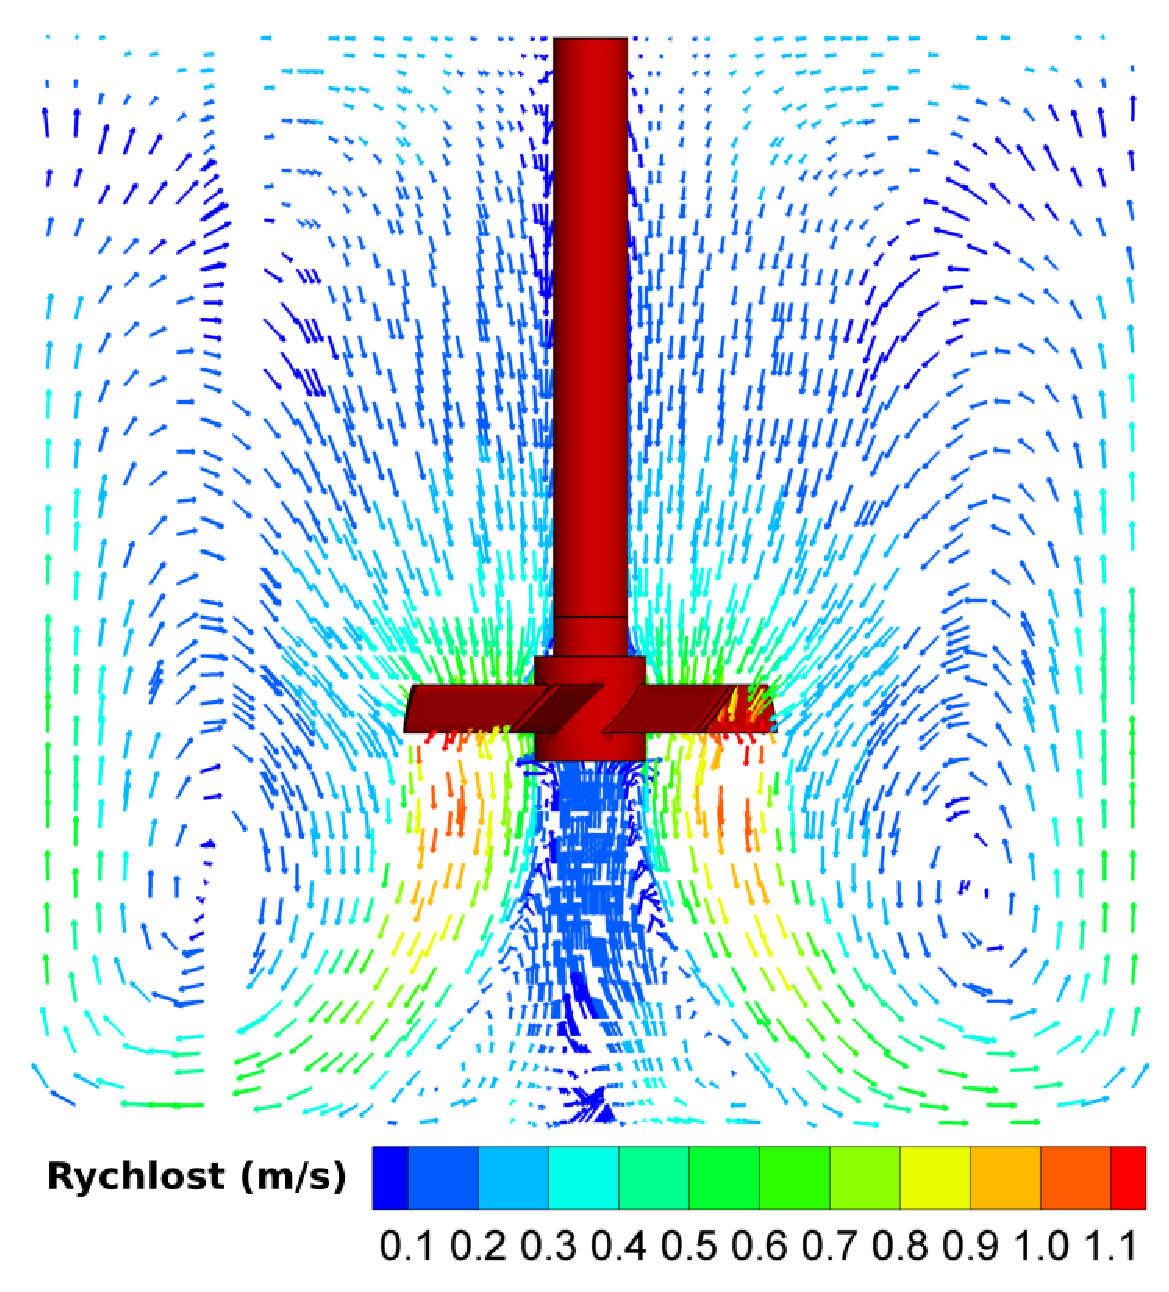
\includegraphics[scale=0.38]{Results/Velocity/keps-std.eps}}  
  \qquad 
  \subfloat[RNG \keps{}]{\label{fig:rng}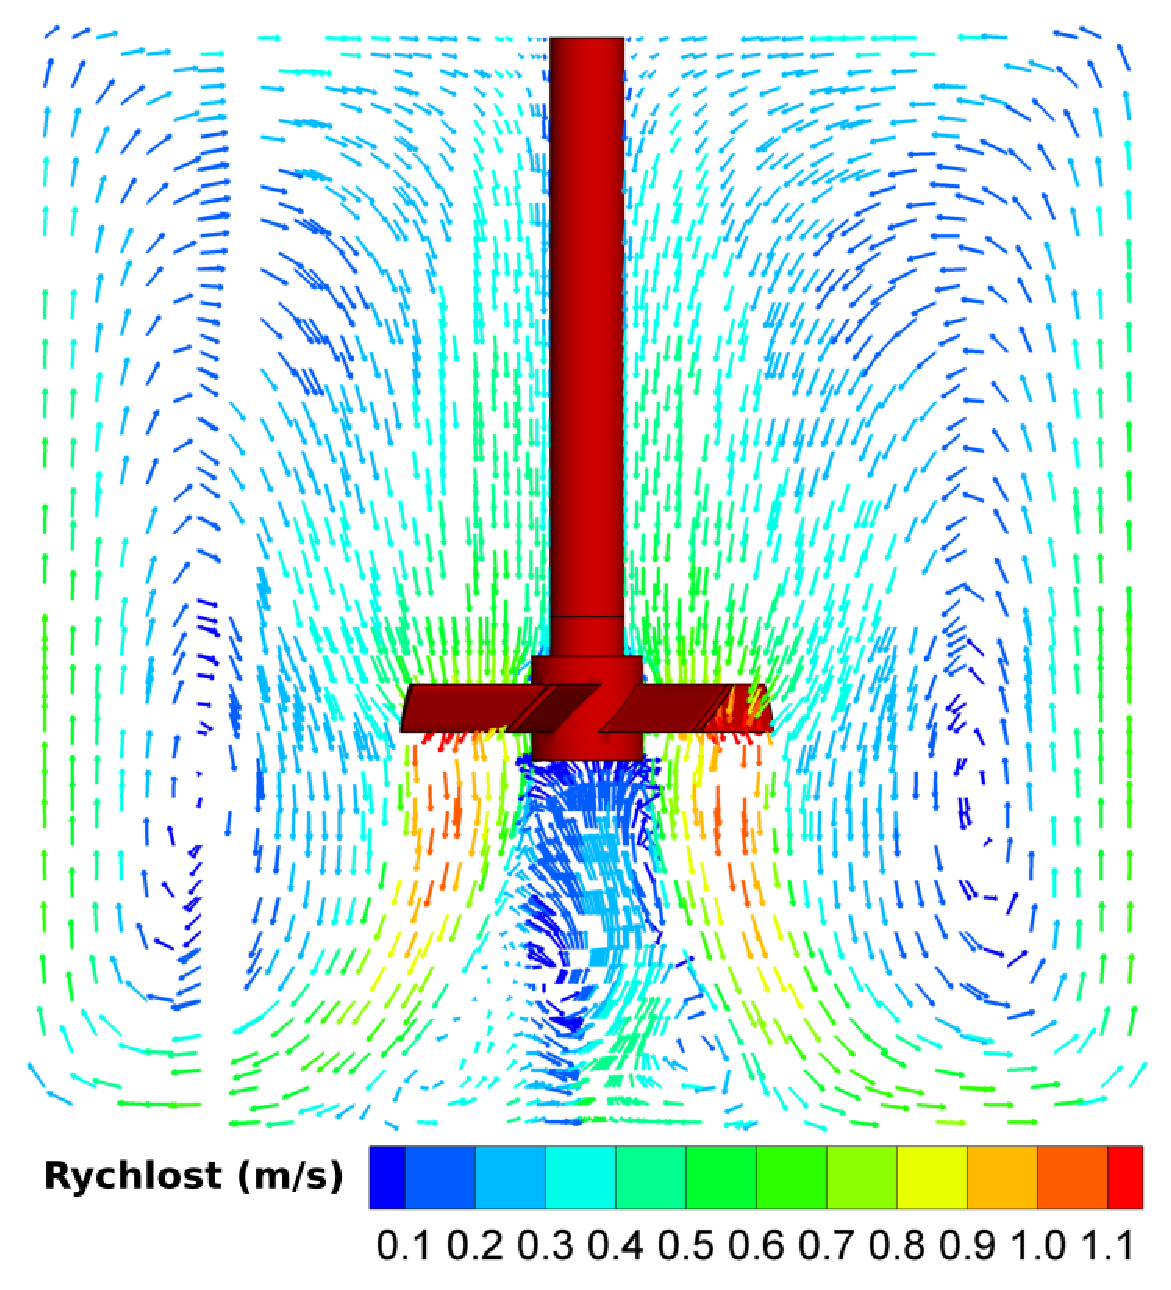
\includegraphics[scale=0.38]{Results/Velocity/keps-RNG.eps}}
\end{figure}
\newpage
\begin{figure}[t!]
  \addtocounter{subfigure}{2}
 \centering
  \subfloat[Realisable \keps{} ]{\label{fig:real}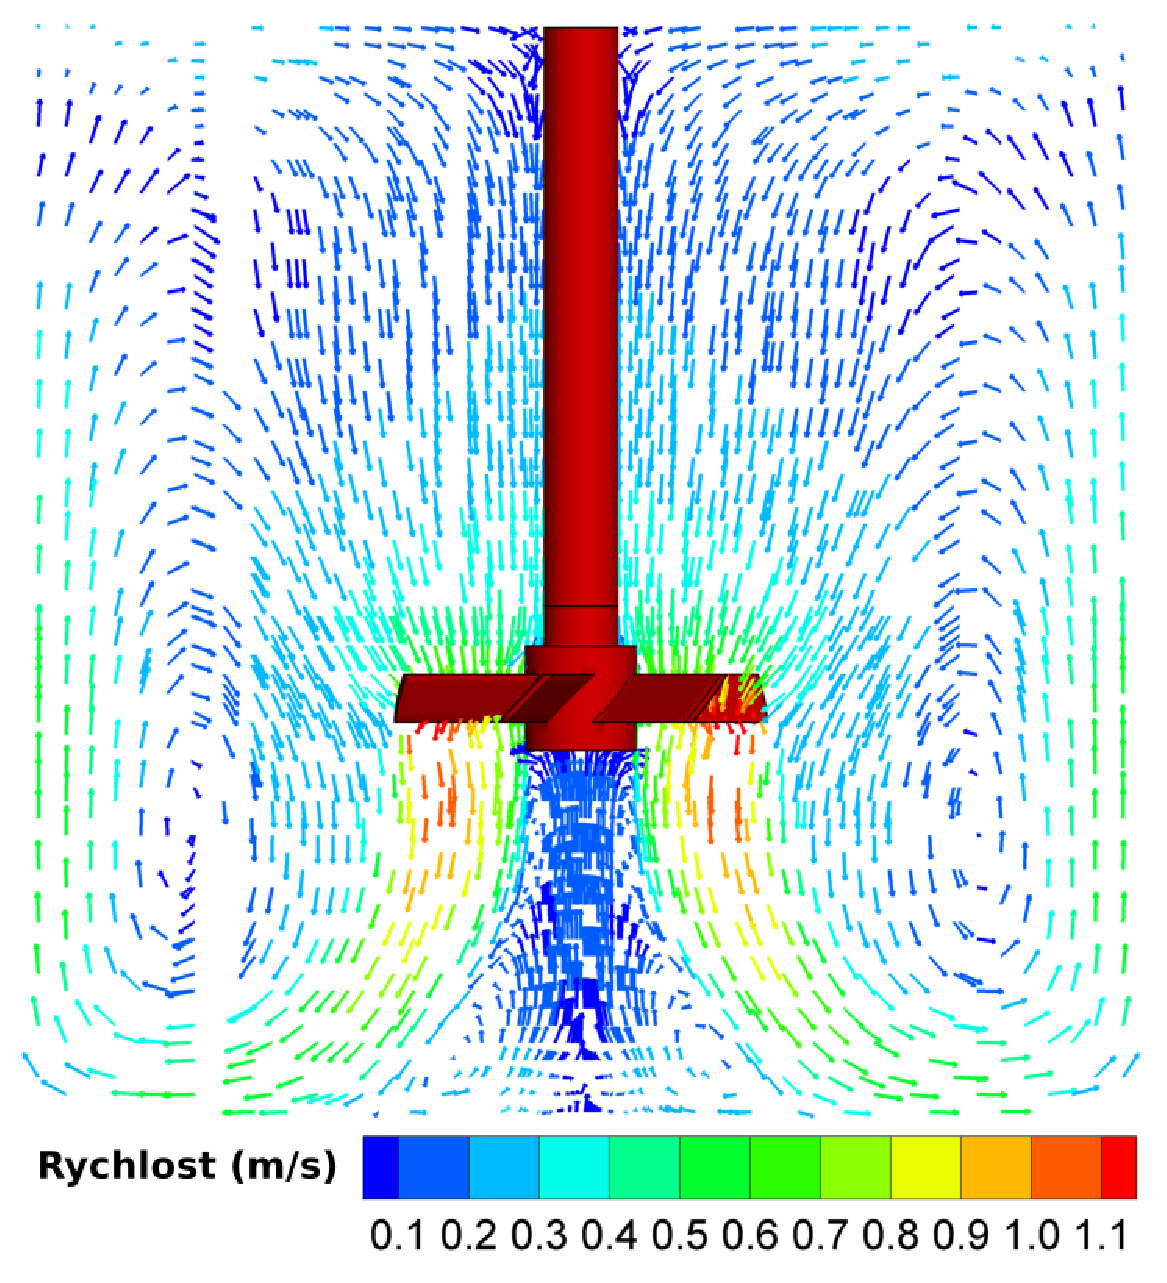
\includegraphics[scale=0.38]{Results/Velocity/keps-real.eps}}
  \qquad
  \subfloat[Standardní RMS]{\label{fig:RMS}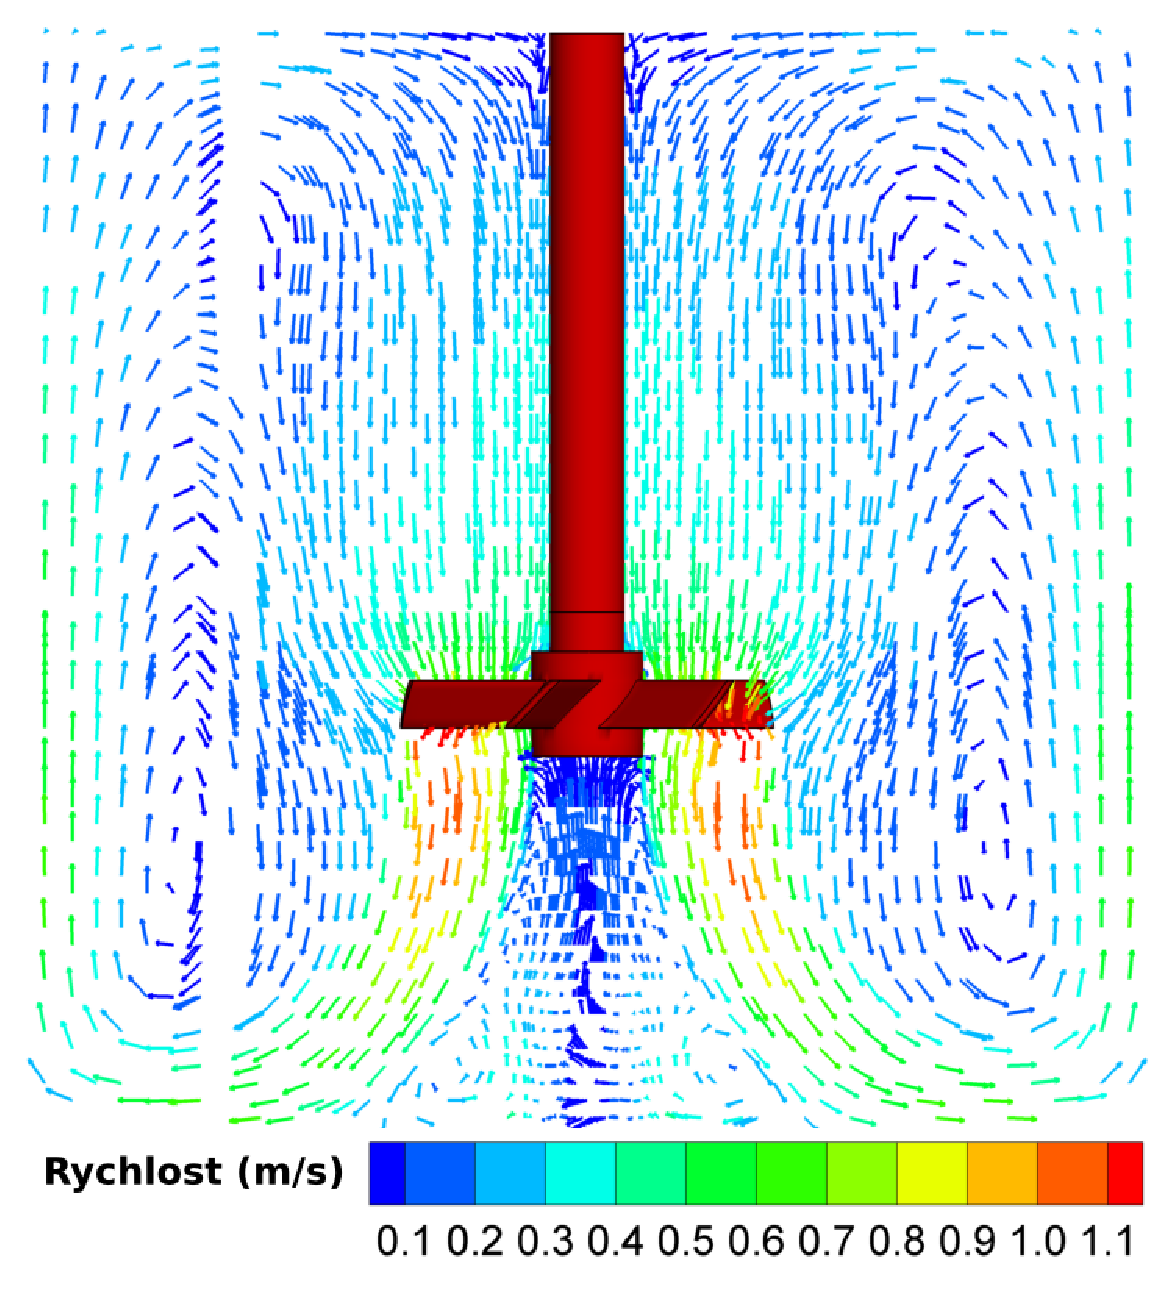
\includegraphics[scale=0.38]{Results/Velocity/RMS.eps}}
  \caption{Vektorové pole rychlosti pro různé turbulentní modely}
  \label{fig:velfield}
\end{figure}

Graf \ref{grf:velfield} zachycuje závislost mezi celkovou rychlostí pohybu kapaliny a vzdáleností ode dna nádoby ($y$) pro jednotlivé turbulentní modely. Konkretní hodnoty pro tento byly získány ve vzdálenosti \SI{0.5}{\centi\meter} podél jedné z narážek nádoby. Z grafu je dobře patrné, že u dna nádrže dochází nárůstu rychlosti tekutiny vlivem působení primární cirkulační smyčky.

\begin{grf}[h!]
 \centering
  \includegraphics[scale=0.45]{Results/Velocity/velField.eps}
  \caption{Průběh velikosti rychlosti tekutiny v nádobě}
  \label{grf:velfield}
\end{grf}

\section{Srovnání modelů pro koeficient odporu}
Jednotlivé modely pro koeficient odporu uvedené v podkapitole \ref{kap:cd} byly porovnány během nestacionární simulace systému obsahující jako vsádku \volproc{5} kuliček z PVC a kapalinu \pvpP. Rychlost otáčení míchadla byla v tomto případě opět nastavena na \SI{7}{\per\second}.

Obr. \ref{fig:cd2} zobrazuje kontury objemového zlomku pevné fáze v~řezu míchací nádobou pro vybrané korelace koeficientu odporu. Tyto údaje byly získány v~času simulace \SI{2}{\second}. 
\begin{figure}[h!]
 \centering

  \subfloat[Schiller-Naumann]{\label{fig:neu2}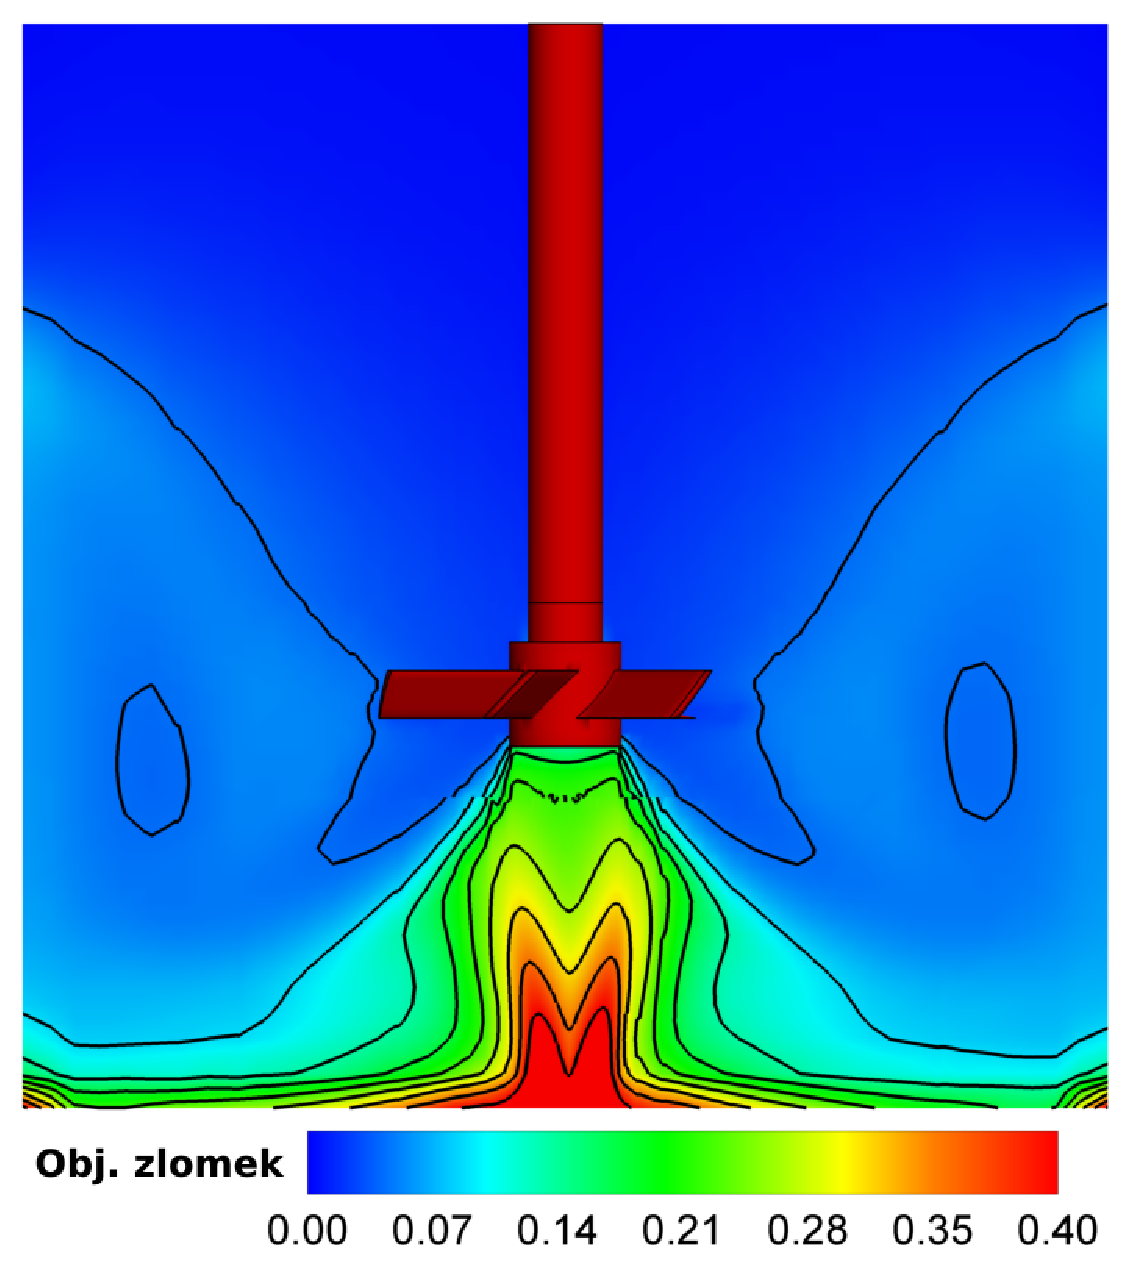
\includegraphics[scale=0.38]{Results/CDComp/neu-2s.eps}}  
  \qquad             
  \subfloat[{Brucato}]{\label{fig:bru2}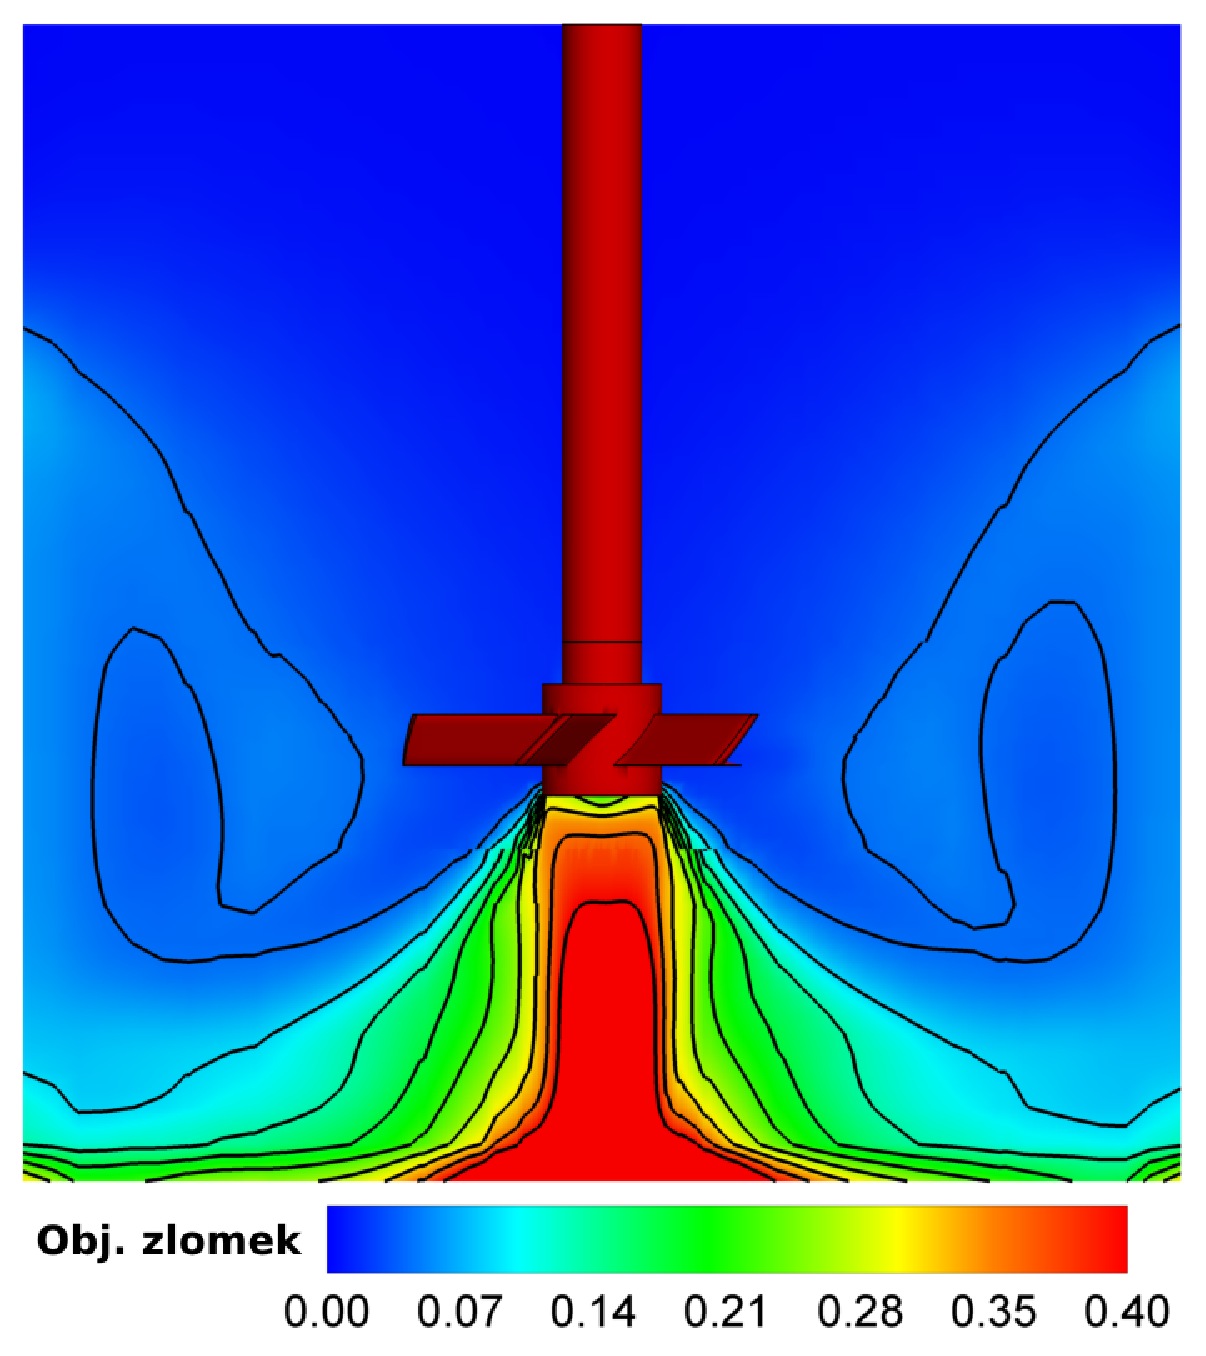
\includegraphics[scale=0.357]{Results/CDComp/bru-2s.eps}}
%\end{figure}
%\newpage
%\begin{figure}[t!]
	%\centering{}
  %\addtocounter{subfigure}{2}
  \\
  \subfloat[{Pinelli}]{\label{fig:pin2}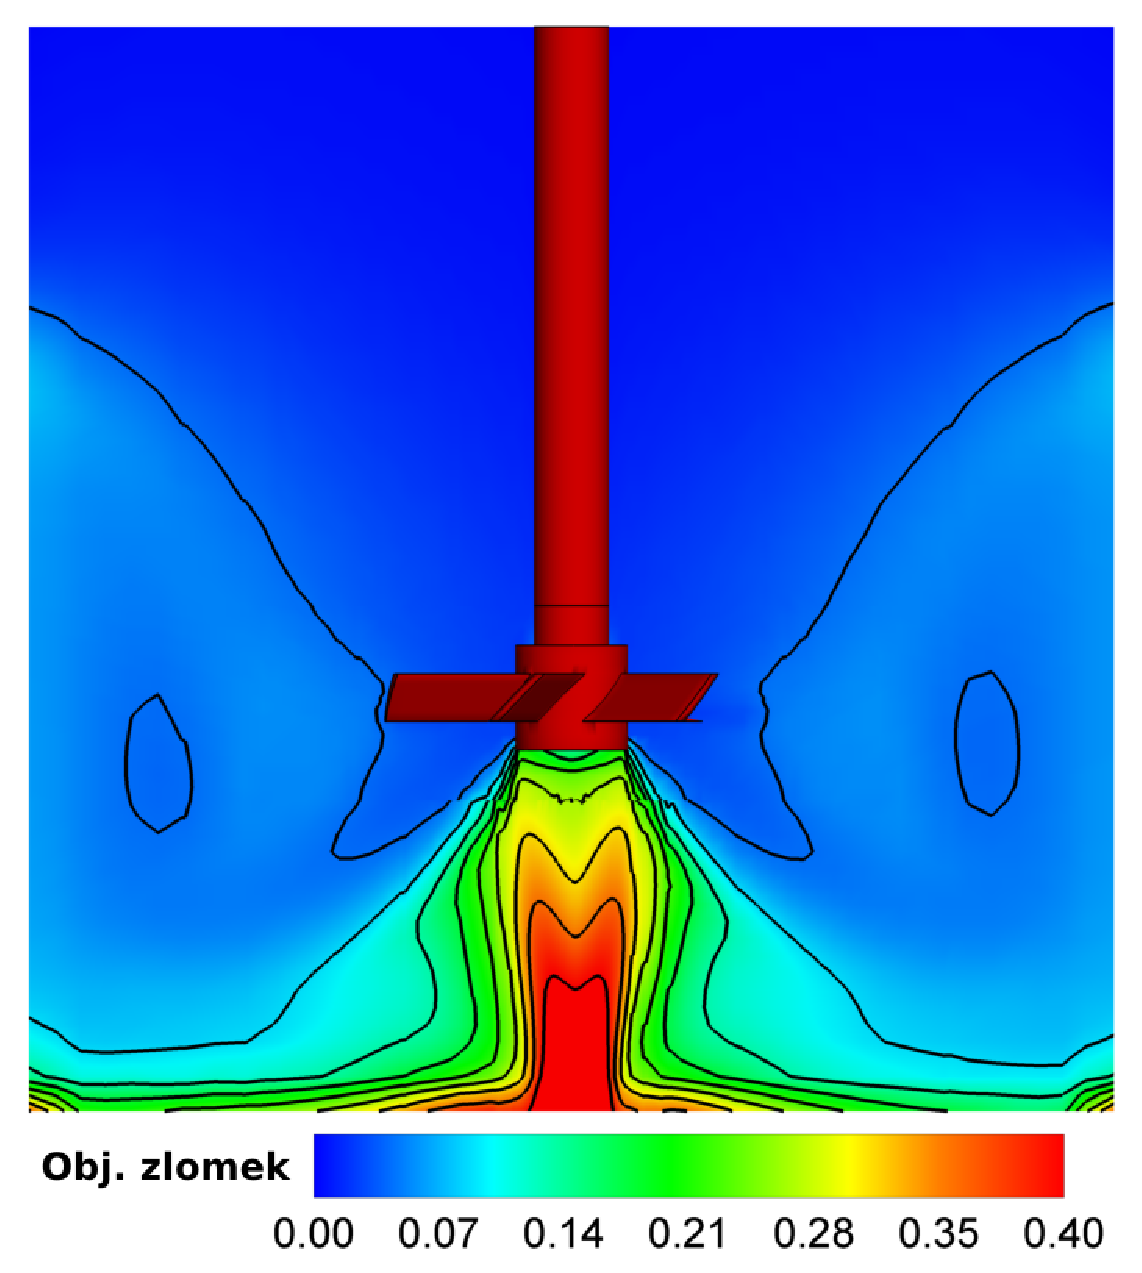
\includegraphics[scale=0.38]{Results/CDComp/pin-2s.eps}}
  \qquad
  \subfloat[{Khopkar}]{\label{fig:kho2}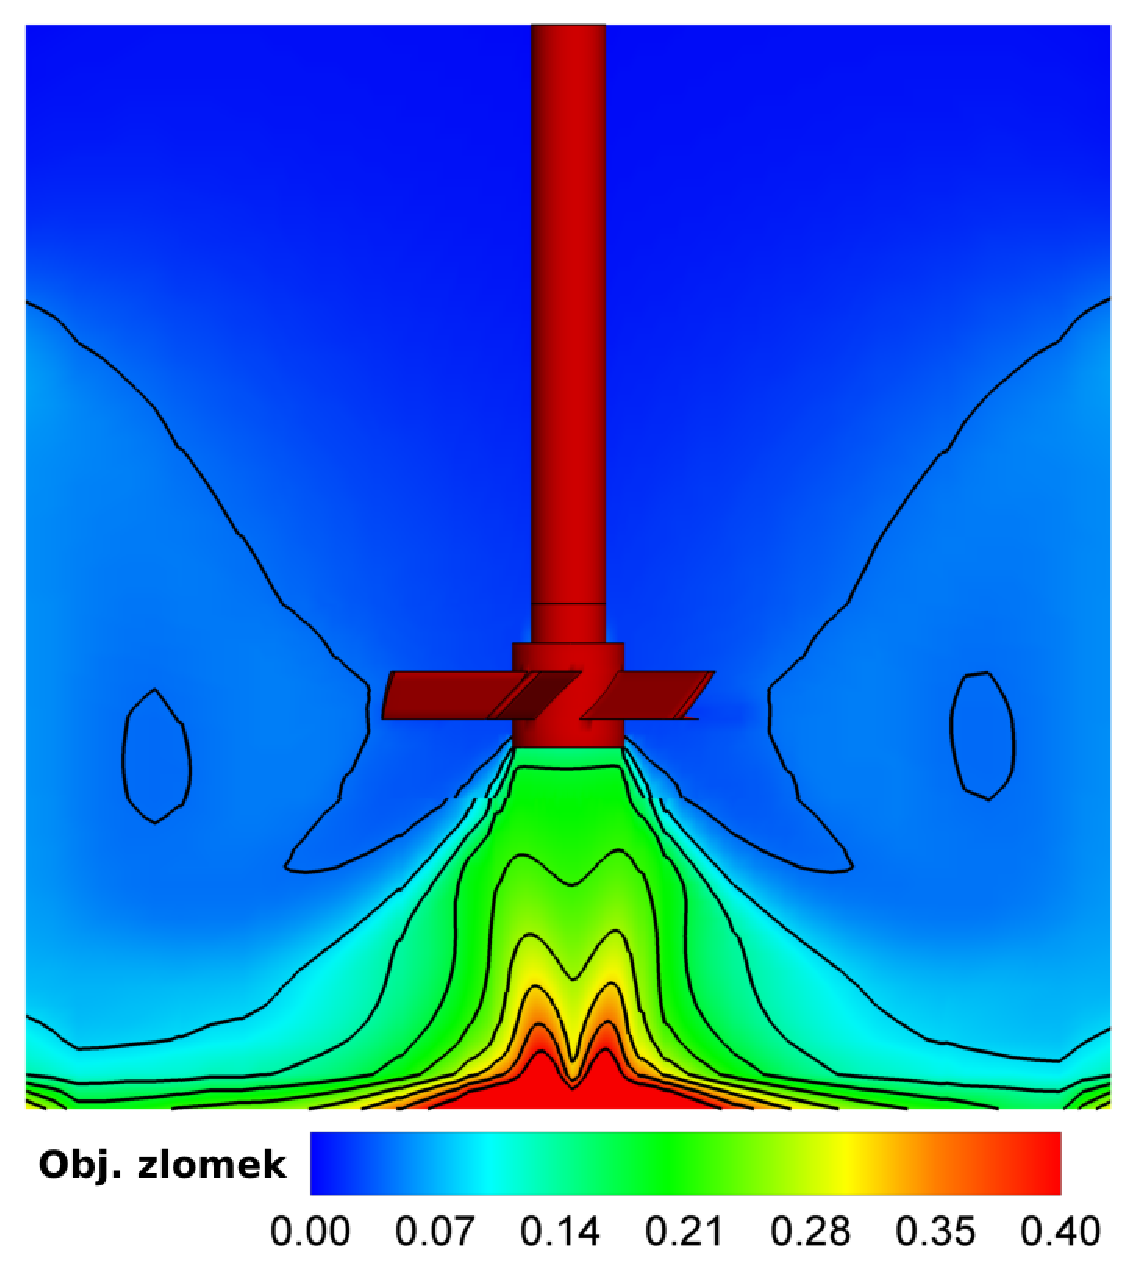
\includegraphics[scale=0.38]{Results/CDComp/kho-2s.eps}}
  \caption{Objemový zlomek pevné fáze v~čase \SI{2}{\second}}
  \label{fig:cd2}
\end{figure}
\newpage
\noindent Z~obrázků je dobře patrné, že přímo pod míchadlem je největší koncentrace pevné fáze vlivem sekundárních cirkulačních smyček, což se podařilo pozorovat i během experimentálního měření.

Série obrázků \ref{fig:cd7} zachycuje objemový zlomek pevné fáze v~řezu nádobou, avšak v čase simulace \SI{7}{\second}. Částice z PVC jsou již značně rozptýleny, ale stále se pod míchadlem nachází oblasti s jejich zvýšenou koncentrací. Nicméně v celé nádobě jsou rozdíly v distribuci pevné fáze mezi jednotlivými modely pro koeficient odporu poměrně zanedbatelné.

\begin{figure}[h!]
 \centering
  \subfloat[Schiller-Naumann]{\label{fig:neu7}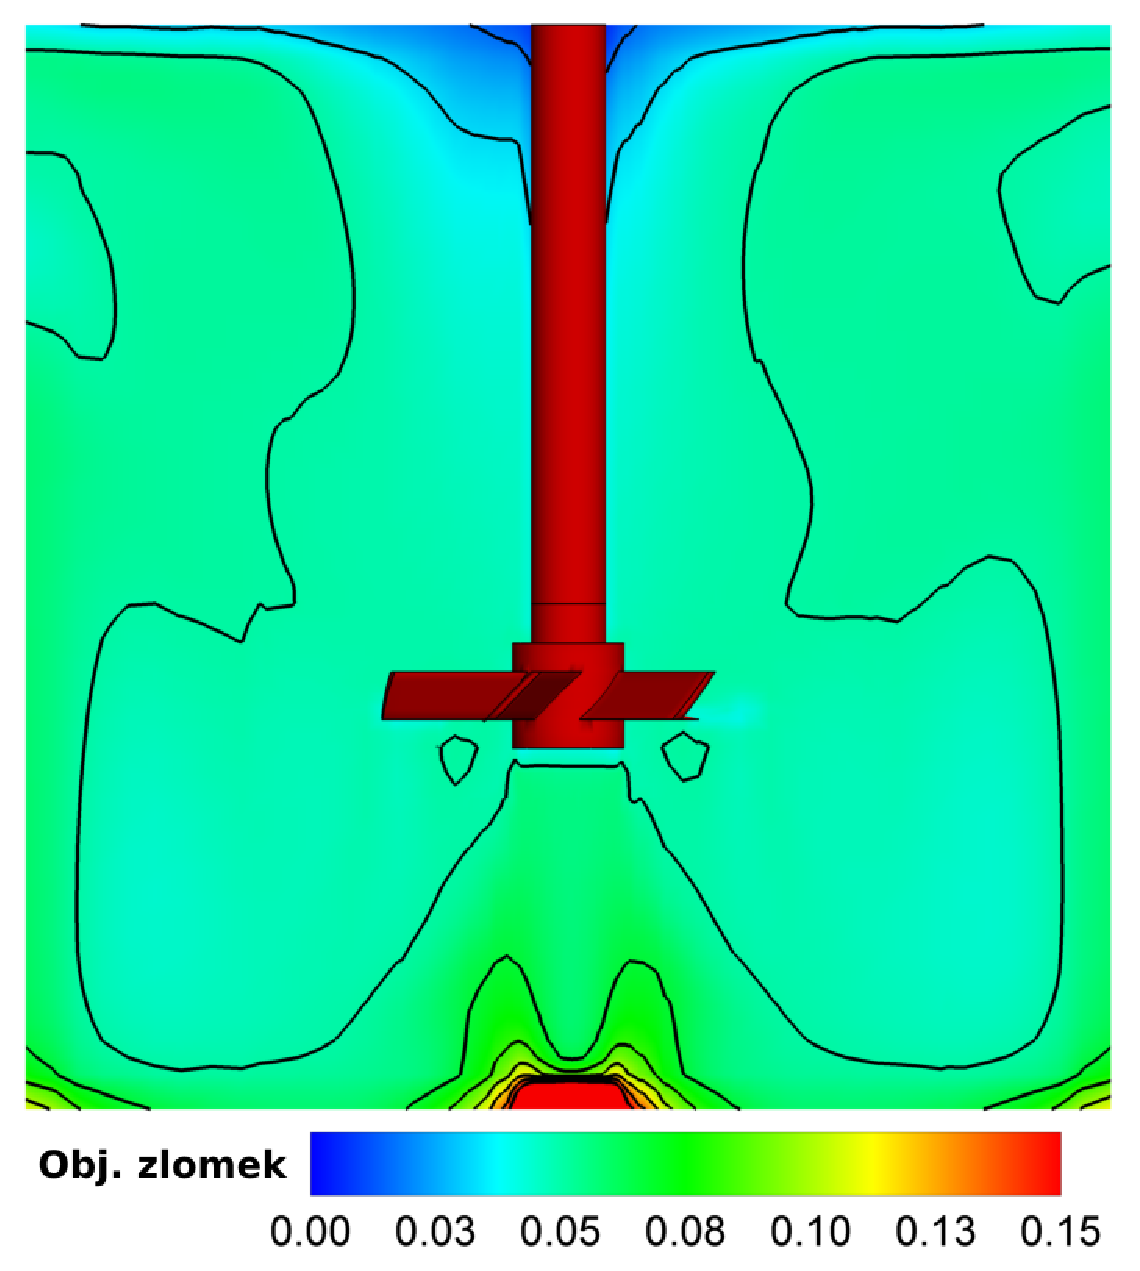
\includegraphics[scale=0.38]{Results/CDComp/neu-7s.eps}}  
  \qquad             
  \subfloat[{Brucato}]{\label{fig:bru7}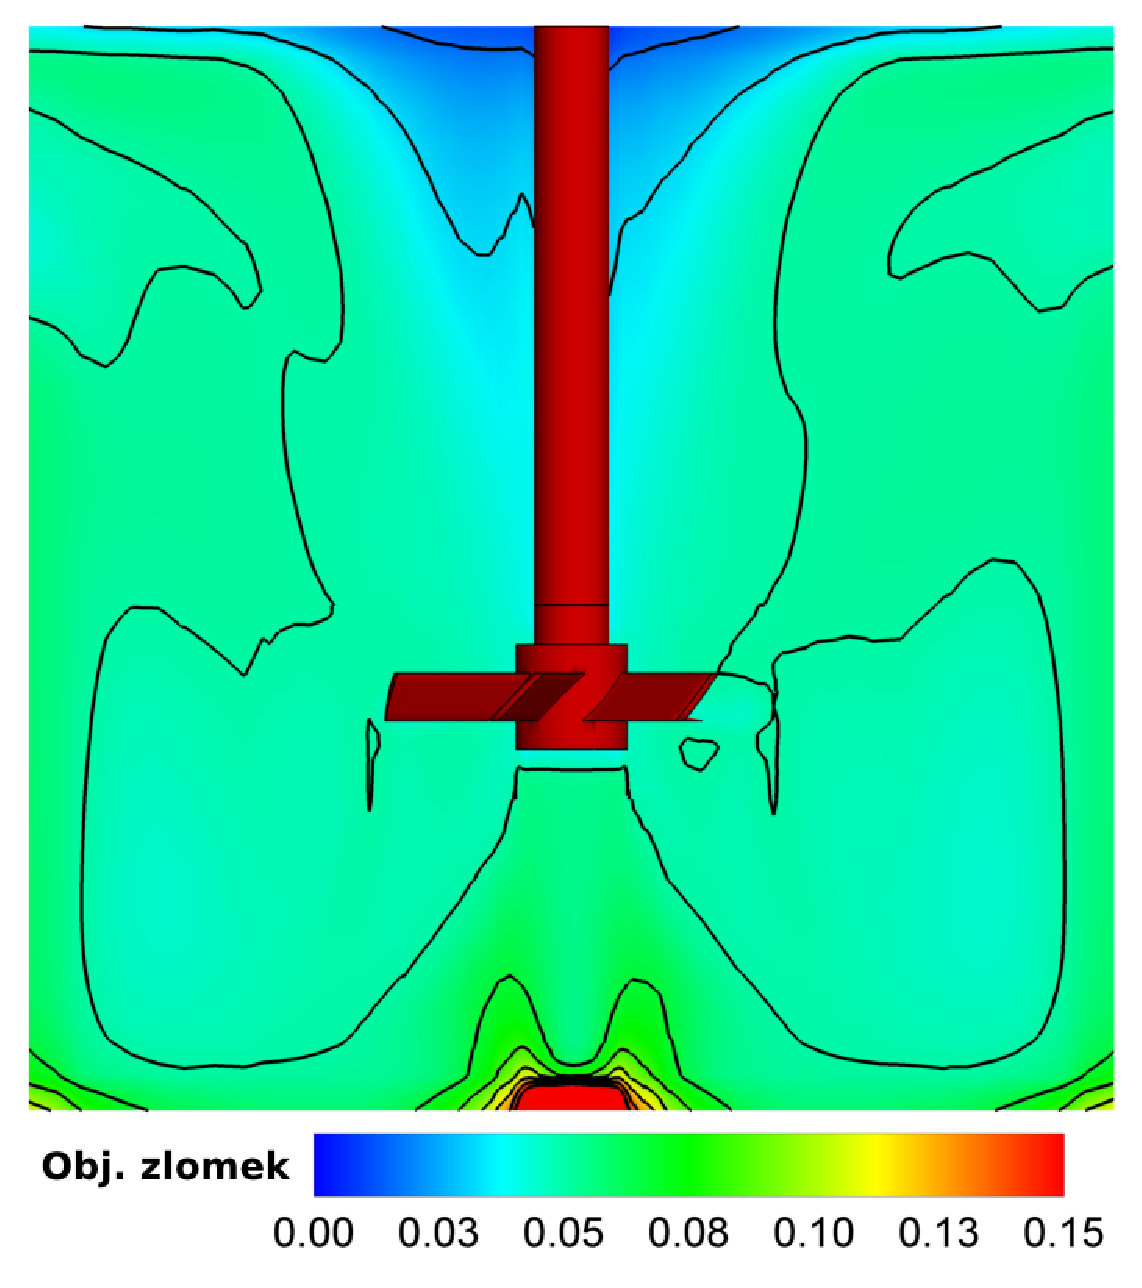
\includegraphics[scale=0.38]{Results/CDComp/bru-7s.eps}}
%\end{figure}
%\newpage
%\begin{figure}[t!]
	 %\centering{}
	 \\
  \subfloat[{Pinelli}]{\label{fig:pin7}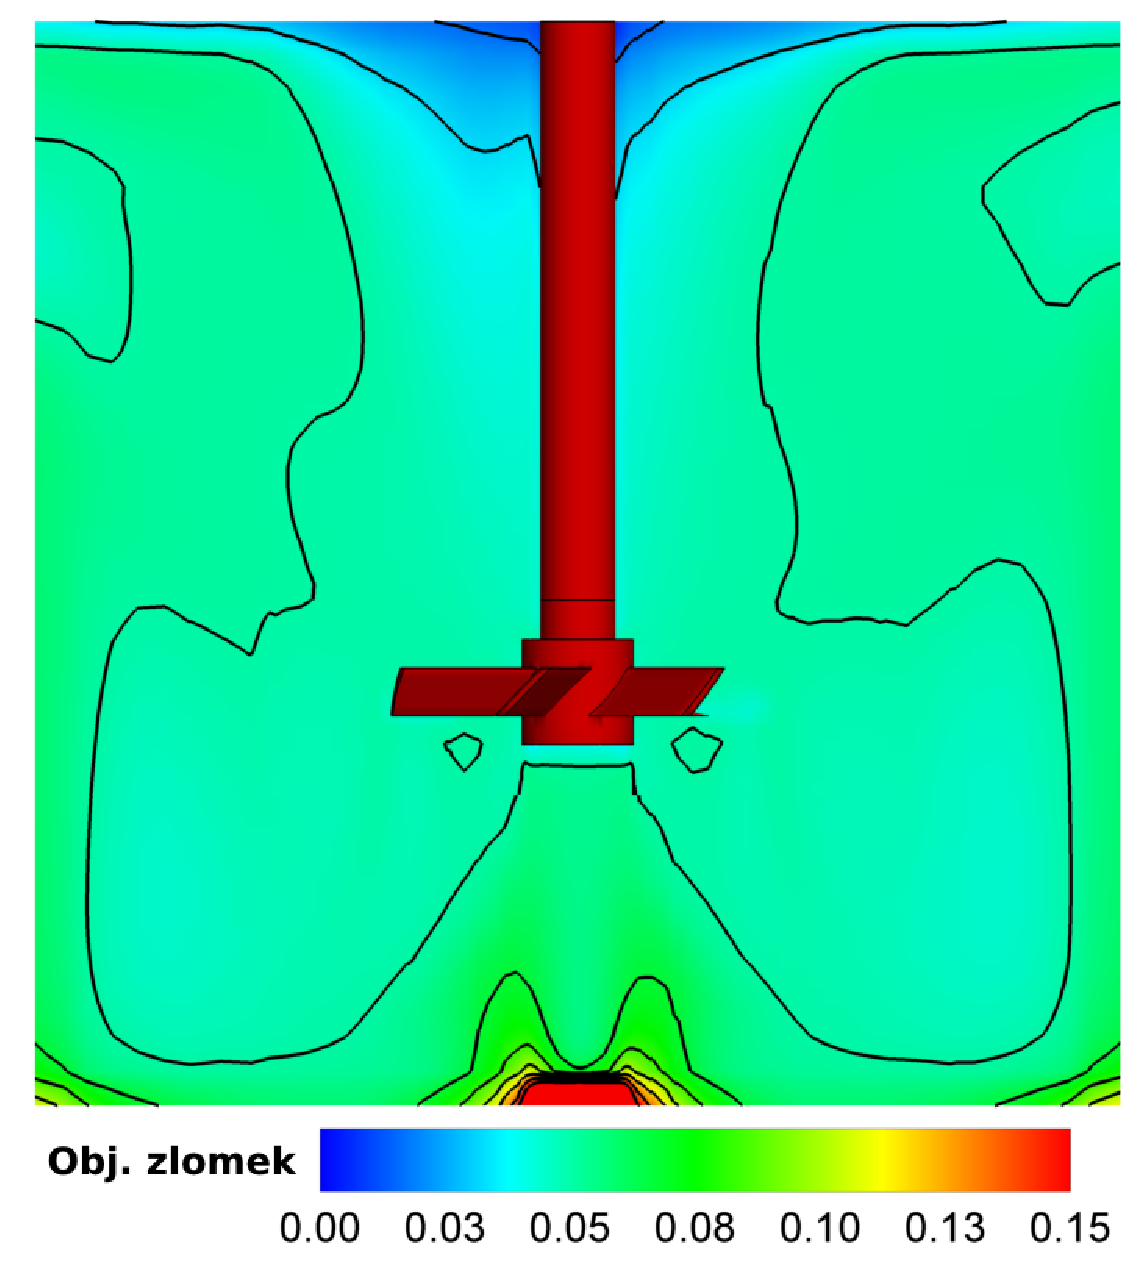
\includegraphics[scale=0.38]{Results/CDComp/pin-7s.eps}}
  \qquad
  \subfloat[{Khopkar}]{\label{fig:kho7}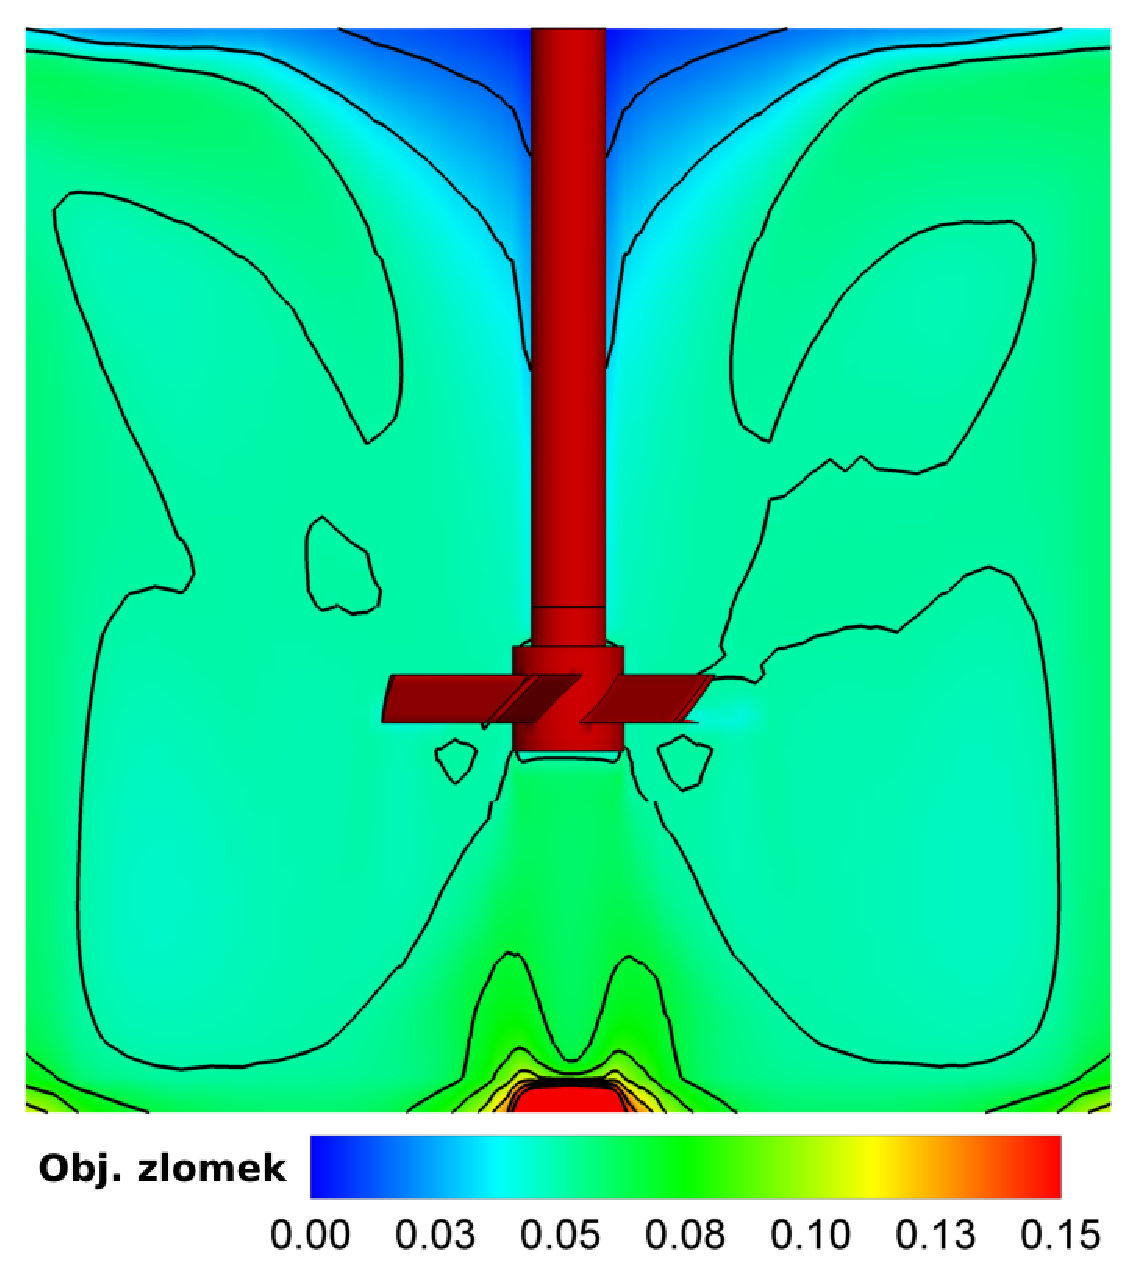
\includegraphics[scale=0.38]{Results/CDComp/kho-7s.eps}}
  \caption{Objemový zlomek pevné fáze v~čase \SI{7}{\second}}
  \label{fig:cd7}
\end{figure}
\newpage
\vspace{-5mm}
Dále jsou zde uvedeny grafické závislosti objemového zlomku pevné fáze na vzdálenosti ode dna nádoby. Z grafu \ref{fig:vol-2} lze vidět, že s~rostoucí vzdáleností se koncentrace pevné fáze postupně snižuje. Avšak grafická závislosti nemá monotonní průběh, přičemž dochází k~tvorbě esovitého koncentračního profilu. Model koeficientu odporu navržený Brucatem předpovídá nižší koncentraci pevné fáze ve vyšší vzdálenosti ode dna než zbylé tři modely. V~čase \SI{7}{\second} kuličky z~PVC již dosáhly značného vznosu a rozdíly mezi jednotlivými korelace pro koeficient odporu se začínaly vytrácet (viz. graf \ref{fig:vol-7}).
\begin{grf}[h!]
 \centering
  \subfloat[v~čase \SI{2}{\second}]{\label{fig:vol-2}\includegraphics[scale=0.39]{Results/CDComp/vol-2s.eps}} 
  \\ 
  \subfloat[v~čase \SI{7}{\second}]{\label{fig:vol-7}\includegraphics[scale=0.39]{Results/CDComp/vol-7s.eps}}
  \caption{Průběh objemového zlomku pevné fáze}
  \label{fig:vol}
\end{grf}
\newpage

Poslední skupina grafů \ref{fig:cd} zachycuje průběh normalizované hodnoty koeficientu odporu v závislosti na světlé výšce. Tato normalizace vznikla vydělením koeficientu odporu jeho průměrnou hodnotou v celé nádrži. Údaje v těchto grafech byly stanoveny podél úsečky v blízkosti radiální narážky.  V~obou případech má  koeficientu odporu podobný průběh pro různé korelace, nicméně v čase \SI{7}{\second} (graf \ref{fig:cd-2}) je zřejmé, že korelace dle Brucata se opět nejznatelněji odlišuje.

\begin{grf}[h!]
 \centering
  \subfloat[v~čase \SI{2}{\second}]{\label{fig:cd-2}\includegraphics[scale=0.40]{Results/CDComp/cd-2s.eps}} 
  \\ 
  \subfloat[v~čase \SI{7}{\second}]{\label{fig:cd-7}\includegraphics[scale=0.40]{Results/CDComp/cd-7s.eps}}
  \caption{Průběh objemového zlomku pevné fáze}
  \label{fig:cd}
\end{grf}
\newpage

